\documentclass[11pt]{scrartcl}
\usepackage[sexy]{{style_files/evan}}

\usepackage{{style_files/NMC}}
\usepackage[subpreambles=true]{standalone}
\usepackage{import}

\begin{document}
\title{NMC Problem Solutions \#2}
\date{Sep. 10, 2022} 
\maketitle

\section*{Welcome!}
    This document contains the solutions to the problems shown in the previous NMC problem set. We recommend not to check the solution to one particular problem unless you already tried it and ran out of ideas.\\
    We tried to make the solutions understandable and hope that you can see where each idea comes from. Keep in mind that the main idea of the problem is usually more important than the technical details.\\
    In any case, if you have trouble reading one (a passage is not clear, or you don't understand how someone could come up with one), just ask us!
    
\section{Algebra}

\textit{
    \begin{flushright}This is the field you're probably the most familiar with. It talks about\\
    \textbf{equations}, \textbf{inequalities}, \textbf{real} (and sometimes complex!) \textbf{numbers}, \textbf{polynomials}...\\
    despite your experience, these problems will require you to think\\
    in new ways not taught in class.\\
    Have fun and think creatively!\end{flushright}
}

\begin{enumerate}[label=\textbf{A\arabic*}.]
    \item Instead of calculating directly what portion of the cake each mathematician gets, let's focus on how much more (or less) cake the $(k+1)$\textsuperscript{th} mathematician gets with respect to the $k$\textsuperscript{th} mathematician. They get to eat $\frac{k+1}{k}$ more fraction of the remaining cake, but the remaining cake is just $\frac{n-k}{n}$ of what it was before. So the $(k+1)\textsuperscript{th}$ mathematician gets more than the $k$\textsuperscript{th} mathematician if and only if \[ \frac{k+1}{k} \cdot \frac{n-k}{n} > 1. \] This rewrites to $(k+1)(n-k) > nk$, which itself rewrites to $-k^2 + n - k > 0$, so $n > k(k+1)$. Note that $k(k+1)$ has a point where it flips from being less than $n$ all the time to being greater than $n$ all the time. So the $(k+1)$\textsuperscript{th} mathematician stops getting more than the $k$\textsuperscript{th} for the smallest $k$ such that $n \le k(k+1)$. For $n = 10\,000$, this ends up being $k=100$, so the $\boxed{100\text{\textsuperscript{th}}}$ mathematician gets the most cake.
\end{enumerate}

\newpage
\section{Combinatorics}
\textit{\begin{flushright}
Combinatorics is a branch of mathematics that primarily deals with\\
\textbf{counting} things in efficient ways, but here we also include \textbf{games}\\
and other creative problems that don't fit in the other categories.\\
Enjoy this playful chapter!
\end{flushright}}

\begin{enumerate}[label=\textbf{C\arabic*}.]
    \item \begin{enumerate}
        \item To see the strategy emerging, we can work backwards: if you are at $0$ pockies than the other person has taken the last pocky, so $0$ pockies is losing. But at $1$, $2$ or $3$ pockies you are winning because you can get to $0$ pockies. At $4$ pockies, however, you are forced to get to either $1$, $2$ or $3$ pockies for your opponent to get to $0$. Continuing in this fashion, $5, 6, 7$ can get to the losing $4$ and $8$ has to go to a winning number of pockies, et cetera.
        
        We observe that all multiples of $4$ seem to be losing numbers of pockies, and we can prove that using the strategy just described: if you are at a multiple of $4$ you have to reduce to a non-multiple of $4$ (and so can never get the last pocky and win on that move), but if you are at a non-multiple of $4$ you \textit{can} always get to a multiple of $4$. After all, if you are at $4k+4$ then you have to reduce to $4k+1, 4k+2, 4k+3$. And if you are at one of those non-multiples of $4$ you can always get to $4k$.
        
        Since there are $30$ pockies, the starting player wins by reducing to $28 = 4 \cdot 7$, so $\boxed{\text{Lance}}$ wins.
    
        \item Let $f(n)$ be the number of ways to finish the box. A player can either take $1$ pocky or $2$ pockies, and then we respectively have $f(n-1)$ and $f(n-2)$ ways left to finish the box. So $f(n) = f(n-1) + f(n-2)$, which exactly matches the Fibonacci numbers in problem \textbf{\hyperref[NT]{N1}}! Now $f(0) = 1$ and $f(1) = 1$, so $f(n) = \boxed{F_{n+1}}$, where $F_n$ is the $n$\textsuperscript{th} Fibonacci number with $F_0 = 0$ and $F_1 = 1$. \label{C1b}
        
        \item We can work backwards again but now keeping track of the losing and winning number of pockies for both parties. It then turns out that $\boxed{\text{MPK}}$ has the winning strategy by first taking $2$ pockies to leave $8$: then Frog, Lance and Arky have to take anywhere between $3$ and $6$ to leave somewhere between $2$ and $5$. Now, if there are $2$ or $3$ pockies, MPK can reduce to $1$, and if there are $4$ or $5$ pockies, MPK can reduce to $3$. In either case, there will be $3$ or less pockies leftover, so the team has to take the last pocky to lose.
        
        \item This is a hard problem and has actually been given a name: Nim. To get a feeling for the problem, you can brute-force some losing triples $(n_1, n_2, n_3)$ using the following rules:
        \begin{enumerate}
            \item $(0,0,0)$ is losing.
            \item If a triple can be moved to a losing triple, it is winning.
            \item If a triple can not be moved to a losing triple, it is losing.
        \end{enumerate}
        For $n_1 + n_2 + n_3 \le 10$, this yields the following losing triples:
        \begin{table}[]
\centering
\begin{tabular}{cccccc}
(0,0,0)   & (1,4,5)  & (2,10,8) & (4,4,0) & (6,3,5) & (8,2,10)  \\
(0,1,1)   & (1,5,4)  & (3,0,3)  & (4,5,1) & (6,4,2) & (8,8,0)   \\
(0,2,2)   & (1,6,7)  & (3,1,2)  & (4,6,2) & (6,5,3) & (8,9,1)   \\
(0,3,3)   & (1,7,6)  & (3,2,1)  & (4,7,3) & (6,6,0) & (8,10,2)  \\
(0,4,4)   & (1,8,9)  & (3,3,0)  & (5,0,5) & (6,7,1) & (9,0,9)   \\
(0,5,5)   & (1,9,8)  & (3,4,7)  & (5,1,4) & (7,0,7) & (9,1,8)   \\
(0,6,6)   & (2,0,2)  & (3,5,6)  & (5,2,7) & (7,1,6) & (9,3,10)  \\
(0,7,7)   & (2,1,3)  & (3,6,5)  & (5,3,6) & (7,2,5) & (9,8,1)   \\
(0,8,8)   & (2,2,0)  & (3,7,4)  & (5,4,1) & (7,3,4) & (9,9,0)   \\
(0,9,9)   & (2,3,1)  & (3,9,10) & (5,5,0) & (7,4,3) & (9,10,3)  \\
(0,10,10) & (2,4,6)  & (3,10,9) & (5,6,3) & (7,5,2) & (10,0,10) \\
(1,0,1)   & (2,5,7)  & (4,0,4)  & (5,7,2) & (7,6,1) & (10,2,8)  \\
(1,1,0)   & (2,6,4)  & (4,1,5)  & (6,0,6) & (7,7,0) & (10,3,9)  \\
(1,2,3)   & (2,7,5)  & (4,2,6)  & (6,1,7) & (8,0,8) & (10,8,2)  \\
(1,3,2)   & (2,8,10) & (4,3,7)  & (6,2,4) & (8,1,9) & (10,9,3)  \\
          &          &          &         &         & (10,10,0)
\end{tabular}
\end{table}

\pagebreak

    Triples like $(7, 4, 3)$ or $(5, 4, 1)$ or $(10, 3, 9)$ look suspicious and remind us of binary. After all, $(7, 4, 3)$ are all powers of $2$ or one below and $3 + 4 = 7$ and $1 + 4 = 5$. And what about $(10, 3, 9)$ in binary? This becomes
    \[
        \begin{bmatrix} 10 \\ 3 \\ 9 \end{bmatrix} = 
        \begin{bmatrix} 1 & 0 & 1 & 0 \\ 0 & 0 & 1 & 1 \\ 1 & 0 & 0 & 1 \end{bmatrix}
    \]
    We now see all the ones `cancelling' each other out! Just like with $(7,4,3)$ or $(5,4,1)$ or any other triple such as $(6, 5, 3)$. To recap our findings, we define the $\textit{bitxor}$: it is an operator $\oplus$ such that $x \oplus y$ in binary gives a $1$ on a given position if and only if exactly one of $x$ and $y$ have a $1$ on that position. For example, $101_2 \oplus 11_2 = 110_2$. We now claim that $(n_1, \ldots, n_k)$ is losing for the starting player if and only if $n_1 \oplus n_2 \oplus \cdots \oplus n_k = 0$. This requires two statements to be proven, just like how we obtained our table of triples before:
    \begin{enumerate}
        \item If $n_1 \oplus \cdots n_k = 0$, then all possible moves to $m_1, \ldots, m_k$ will have $m_1 \oplus \cdots \oplus m_k \ne 0$.
        \item If $n_1 \oplus \cdots n_k \ne 0$, then there exists a move such that $m_1 \oplus \cdots \oplus m_k = 0$.
    \end{enumerate}
    If these statements are true, then one player can always force $n_1 \oplus \cdots \oplus n_k \ne 0$ for themselves, which means eventually the game will end up with $0 \oplus \cdots \oplus 0 = 0$, which ends up at the other player, and as such the player with $n_1 \oplus \cdots \oplus n_k \ne 0$ must have been the one having picked the last pocky.
    
    For the first statement, note that if we replace a number $n_i$ by $m_i < n_i$, then there has been changed at least one digit by uniqueness of writing an integer in binary. If we now compare $n_1 \oplus \cdots \oplus n_k$, with $m_1 \oplus \cdots \oplus m_k$, then no number has been changed in the bitxor except $m_i$, where the at least one digit change leads to a digit change at the bitxor on the same position (as the parity of the number of ones changes there). So \[ m_1 \oplus \cdots \oplus m_k  \ne n_1 \oplus \cdots \oplus  n_k = 0, \] which we wanted to prove.
    
    For the second statement we are already done if we can find an $i \in \{1, \ldots, k\}$ such that \[ n_i > n_i \oplus (n_1 \oplus n_2 \oplus \cdots \oplus n_i \oplus \cdots \oplus n_k). \] After all, then we can pick $m_i$ equal to the right hand side such that \[ m_1 \oplus m_2 \oplus \cdots \oplus m_k = (n_1 \oplus \cdots \oplus n_k) \oplus (n_1 \oplus \cdots \oplus n_k) = 0 \] since $\oplus$ is associative and commutative, and $x \oplus x = 0$ for all $x$.
    
    So we want to find an $n_i$ with a $1$ on the highest (leftmost) $1$ of $n_1 \oplus \cdots \oplus n_k$, such that highest changed bit in $n_i \oplus (n_1 \oplus \cdots \oplus n_k)$ with respect to $n_i$ is a $1$ to $0$, such that the inequality immediately holds (since in any base we can compare two digits by comparing the most significant, leftmost, difference in digits). But in $n_1 \oplus \cdots \oplus n_k$ a bit is $1$ if and only if there is an odd number and as such positive number of $n_j$'s with a $1$ on its position, so we can indeed such an $n_i$.
    
    So boxes with $n_1, \ldots, n_k$ pockies wins for the starting player Arky if and only if $n_1 \oplus n_2 \cdots \oplus n_k \ne 0$.
    \end{enumerate}
    \end{enumerate}
    

\newpage
\section{Geometry}
\textit{\begin{flushright}
Geometry, studied since ancient Greece, is the oldest discipline of mathematics. It concerns \textbf{space}, \textbf{distances}, \textbf{areas}, \textbf{volumes}.\\ Learn the pretty intricacies of the figures below!
\end{flushright}}

\begin{enumerate}[label=\textbf{G\arabic*}.]
    \item \begin{enumerate}
        \item In an isosceles triangle, we know that from the top vertex the angle bisector is the same as median. So we can use that by intersecting a circle centered at $O$ in $X$ and $Y$ at $OA$ and $OB$ respectively. Then the angle bisector passes through the midpoint of $XY$, and also $O$. But both points are of equal distance to $X$ and $Y$, so the angle bisector is also the perpendicular bisector of $XY$ (since it is the line of points that are of equal distance to both $X$ and $Y$). We can construct that by constructing two points of equal distance to $X$ and $Y$, for example by intersecting the circle with center $X$ through $Y$ with the circle with center $Y$ through $X$ and drawing a line through the intersection points.
        
        \begin{center}
        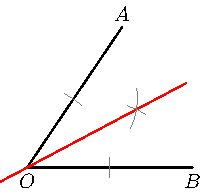
\includegraphics[width = 5cm, page = 1]{Diagrams/W2G1sol.pdf}
        \end{center}
        
        \item This line actually just needs to cut through the center $O$ of rectangle $ABCD$: the resulting two rectangle halves are then symmetric in $O$, so they have equal area. We can construct this center by intersecting lines $AC$ and $BD$.
        
        \begin{center}
        \includegraphics[width = 5cm, page = 2]{Diagrams/W2G1sol.pdf}
        \end{center}
        
        \item Note that a circle is defined as the collection of points all of equal distance to its center. So if we pick two points $A$ and $B$ on the circle with center $O$, then $OA = OB$. So $O$ lies on the perpendicular bisector of $AB$. This means that we can construct two perpendicular bisectors of two chords (line segments starting and ending on the circle) and let them intersect on the circle.
        
        We can do this efficiently by picking a random point $A$ on the circle, then constructing a (small enough for two intersection points) circle centered at $A$ intersecting the circle $c_1$ at $B$ and $C$, then constructing the circles $c_2$ and $c_3$ with center $B$ and $C$ through $A$. Then the intersection points of $c_1$ and $c_2$ go through the perpendicular bisector of $AB$, and the intersection points of $c_2$ and $c_3$ go through the perpendicular bisector of $AC$. This construction will only end up costing five circles and lines in total.
        
        \begin{center}
        \includegraphics[width = 5cm, page = 3]{Diagrams/W2G1sol.pdf}
        \end{center}
    \end{enumerate}
\end{enumerate}

\newpage
\section{Number Theory} \label{NT}
\textit{\begin{flushright}
Number theory is the part of mathematics that deals with the\\ \textbf{integers} (numbers w/ no decimal dot), \textbf{factorization}, \textbf{divisibility}, \textbf{primes}, ...\\ While its objects are simple, don't be deceived,\\ solutions still require a good bit of cleverness!
\end{flushright}}
\begin{enumerate}[label=\textbf{N\arabic*}.]
    \item \begin{enumerate}
        \item We use Euclid's algorithm: \[ \gcd(a, b) = \gcd(a, b-a). \] Here, $\gcd(a,b)$ denotes the greatest common divisor between two integers $a$ and $b$. To prove $\gcd(a, b) = \gcd(a, b-a)$, we look at the common divisors of $a$ and $b$ and show that these are also exactly the common divisors of $a$ and $b-a$. So suppose we have a $g$ dividing both $a$ and $b$. This means that $a = gj$ and $b = gk$ for some $j$ and $k$. But then $b - a = g(k-j)$, so $g$ is also a divisor of $b-a$. So all common divisors of $a$ and $b$ are also common divisors of $a$ and $b-a$. Similarly, if we have a $g$ dividing both $a$ and $b-a$, then we write $a = gj$ and $b-a = gk$ such that $b = a + (b-a) = g(j+k)$, so $g$ is also a common divisor of $a$ and $b$. So $\gcd(a, b) = \gcd(a, b-a)$, since we are taking the maximum divisor of the exact same divisors.
        
        Now note that two numbers $a$ and $b$ are coprime if and only if $\gcd(a,b) = 1$. After all, if $\gcd(a,b) = 1$ then their greatest divisor is $1$, so it's their only divisor, so $a$ and $b$ are coprime. And if $a$ and $b$ are coprime then their only common divisor is $1$, so $\gcd(a,b) = 1$. (Yes, we are taking just positive divisors here.)
        
        We now have enough to prove the statement in the problem. Note that the GCD between two consecutive Fibonacci numbers $F(n)$ and $F(n+1)$ is equal to
        \[
          \gcd(F(n), F(n+1)) = \gcd(F(n), F(n+1) - F(n)) = \gcd(F(n), F(n-1))
        \]
        using Euclid's algorithm. But this is the GCD between the previous two Fibonacci numbers! Applying Euclid's algorithm a total number of $n$ times, we know that \[ \gcd(F(n), F(n+1)) = \gcd(F(n-1), F(n)) = \cdots = \gcd(F(0), F(1)) = \gcd(0, 1) = 1. \] So $F(n)$ and $F(n+1)$ are coprime for all $n \ge 0$. \label{N1a}
    
       \item Let's take a look at when the Fibonacci numbers are odd ($1$) or even ($0$): \[ 0, 1, 1, 0, 1, 1, 0, 1, 1, 0, \cdots \] This seems to be a periodic sequence that goes $0,1,1$ the entire time. And we can see why this is true: if we have $0,1,1$ then the next number will be an odd number plus an odd number, so it's even. Then the next one will be even plus odd, so odd. And the next one will be even plus odd again, so odd. So we keep having $0, 1, 1$ again. So $F(m)$ is even if and only if $m$ is a multiple of $3$.
       
       What we have done here is focus on the remainders by division by $2$, and in fact if we just care about remainders of a sum of two numbers we can just sum the two remainders together. So for divisibility by $5$ we can focus on the remainders by division by $5$. And in fact we see the following periodic sequence: \[ 0,1,1,2,3,0,3,3,1,4,0,4,4,3,2,0,2,2,4,1, \ldots \] So $F(m)$ is divisible by $5$ is and only if $m$ is divisible by $5$. And for divisibility by $7$ we have the following sequence: \[ 0,1,1,2,3,5,1,6,0,6,6,5,4,2,6,1, \ldots \] So $F(m)$ is divisible by $7$ if and only if $m$ is divisible by $7$.
       
       However, this solution just doesn't feel right. Why do we have a long periodic sequence but more periodic zeroes? For this, we have the following statement: \[ \gcd(F_m, F_n) = F_{\gcd(m,n)}. \]
       
       To prove this, we are going to prove the `Fibonacci' form of Euclid's theorem:
       \[
         \gcd(F_m, F_n) = \gcd(F_m, F_{n-m}).
       \] 
       If this is true, then applying this identity over and over again eventually yields $\gcd(F_m, F_n) = \gcd(F_0, F_{\gcd(m,n)}) = F_{\gcd(m,n)}.$
       
       We are going to prove the following identity first:
       \[
         F_{x+y} = F_{x} F_{y-1} + F_{x+1} F_y.
       \]
       To see this, note that by \textbf{\hyperref[C1b]{C1b}} that $F_t$ is the number of ways to finish a box of $t-1$ pockies while taking $1$ or $2$ pockies each. The left hand side then stands for finishing a box of $x+y-1$ pockies. To do this more creatively, we can either first eat $x-1$ pockies, eat $2$ pockies at once and then eat the rest of $y-2$ pockies. Or we can not eat $x-1$ pockies and end up at $x$ pockies eventually, and then finish the rest of $y-1$. This two-way split of finishing the box exactly matches the right hand side, so the identity is proven.
       
       Now, plugging in $x = n-m$ and $y = m$ into the identity yields
       \[
         F_{n} = F_{n-m} F_{m-1} + F_{n-m+1} F_{m}.
       \]
       So using the Euclidean algorithm we obtain
       \[
         \gcd(F_m, F_n) = \gcd(F_m, F_{n-m} F_{m-1} + F_{n-m+1} F_{m}) = \gcd(F_m, F_{n-m} F_{m-1}),
       \]
       where we subtracted $F_{n-m+1} F_{m}$ since it is a multiple of $F_m$. But now notice that $F_m$ and $F_{m-1}$ are coprime by part \hyperref[N1a]{a}, so a common divisor of both $F_m$ and $F_{n-m} F_{m-1}$ is actually just a common divisor of both $F_m$ and $F_{n-m}$ and vice versa. So $\gcd(F_m, F_n) = \gcd(F_m, F_{n-m})$, like we wanted to prove.
       
       So let's return to divisibility by $5$. We note that $F_1, F_2, F_3, F_4$ are not divisible by $5$ but $F_5$ is. Now, in general we have that
       \[
         \gcd(F_n, F_5) = F_{\gcd(n, 5)}.
       \]
       Now this GCD is divisible by $5$ if and only if $\gcd(n, 5) = 5$ since $\gcd(n,5) \le 5$ and the only positive Fibonacci index $\le 5$ making the Fibonacci number divisible by $5$ was $5$ itself. And since $5 \mid F_5$, we have that the GCD is divisible by $5$ if and only if $5 \mid F_n$. And $\gcd(n,5) = 5$ if and only if $5 \mid n$. So $5 \mid F_n$ if and only if $5 \mid n$.
       
       For divisibility by $7$, we again note that $F_1, \ldots, F_7$ are all not divisible by $7$ but $F_7$ is. Then
       \[
         \gcd(F_n, F_7) = F_{\gcd(n, 7)}
       \]
       is divisible by $7$ if and only if $\gcd(n,7) = 7$, if and only if $7 \mid n$. And the GCD is divisible by $7$ if and only if $7 \mid F_n$. So $7 \mid F_n$ if and only if $7 \mid n$. \label{N1b}
      
      \item Using our identity
      \[
         \gcd(F_m, F_n) = F_{\gcd(m,n)}
       \] 
       from part \hyperref[N1b]{b}, we obtain 
       \[
         \gcd(F_{2n}, F_n) = F_{\gcd(2n,n)} = F_n,
       \] 
       so $F_n$ indeed divides $F_{2n}$.
       
       Alternatively, using 
       \[
         F_{x+y} = F_{x} F_{y-1} + F_{x+1} F_y
       \]
       and plugging in $x = y = n$ we get \[ F_{2n} = F_n(F_{n-1} + F_{n+1}), \] so $F_{2n}$ is divisible by $F_n$.
     
     \item To prove that
     \[
       F(0) + F(1) + \cdots + F(n) = F(n+2) - 1,
     \]
     we are going to use problem \textbf{\hyperref[C1b]{C1b}} again to say that both sides count the same thing.
     
     The right hand side counts the number of ways to finish a box of $n+1$ pockies, minus one way: we will let that one way be just taking $1$ pocky each and every time.
     
     To finish a box of $n+1$ without always taking $1$ pocky each time, we can look at when we first take $2$ pockies: if we do this when there are $k \in \{2, 3, \ldots, n+1\}$ pockies left, then we will have $k-2 \in \{0, 1, \ldots, n-1\}$ pockies leftover. Before taking $2$ pockies for the first time, there is only one possibility to have taken pockies (just $1$ pocky every move), and after taking $2$ pockies, there are $F(k-1)$ ways left. That is, in total we have $F(1) + F(2) + \cdots + F(n)$ ways to finish a box of $n+1$ pockies without taking $1$ pocky each time. Adding $F(0) = 0$ to this yields 
     \[
       F(0) + F(1) + \cdots + F(n) = F(n+2) - 1,
     \]
     as we wanted to show.
    \end{enumerate}
\end{enumerate}

\end{document}
